% 2017_tianjin_science_q17_fig1: pyramid P-ABC, D,E,N,M.
% P apex; PA vertical dashed; base B-N-C solid; BE solid through M.
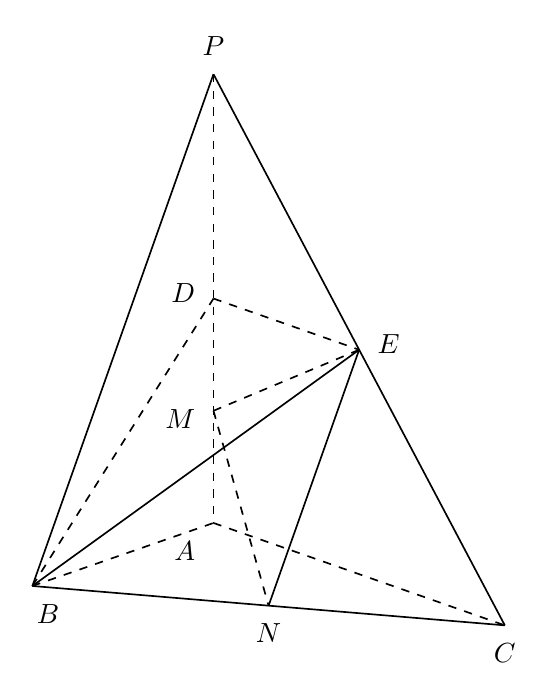
\begin{tikzpicture}[x=1cm,y=1cm,font=\normalsize,line width=.6pt]
\coordinate (P) at (2.3,7);
\coordinate (A) at (2.3,1.3);
\coordinate (B) at (0,0.5);
\coordinate (C) at (6,0);
\coordinate (N) at (3,0.25);
\coordinate (D) at (2.3,4.15);
\coordinate (E) at (4.1500000000,3.5000000000);
\coordinate (M) at (2.3000000000,2.7250000000);
% outer pyramid
\draw[solid,line width=.6pt] (P)--(B);
\draw[solid,line width=.6pt] (P)--(C);
\draw[solid,line width=.6pt] (B)--(C);
\draw[solid,line width=.6pt] (B)--(E);
\draw[solid,line width=.6pt] (E)--(N);



% hidden / interior dashed
\draw[dashed,line width=.6pt] (P)--(A);
\draw[dashed,line width=.6pt] (B)--(A);
\draw[dashed,line width=.6pt] (A)--(C);
\draw[dashed,line width=.6pt] (B)--(D);
\draw[dashed,line width=.6pt] (D)--(E);

\draw[dashed,line width=.6pt] (M)--(N);
% right-angle mark at A (PA perp base)
\node[anchor=south,yshift=3pt] at (P) {$P$};
\node[anchor=east,xshift=-3pt,yshift=2.0pt] at (D) {$D$};
\node[anchor=east,xshift=-3pt,yshift=-3.0pt] at (M) {$M$};
\node[anchor=north east,xshift=-3.0pt,yshift=-3pt] at (A) {$A$};
\node[anchor=north west,xshift=-2.0pt,yshift=-3pt] at (B) {$B$};
\node[anchor=north,yshift=-3pt] at (N) {$N$};
\node[anchor=north,yshift=-3pt] at (C) {$C$};
\node[anchor=west,xshift=3pt,yshift=2.0pt] at (E) {$E$};
\draw[dashed] (M)--(E);
\end{tikzpicture}
